\documentclass[notitlepage,a4paper,twoside,10pt]{article}

\usepackage{mathpazo} 
\usepackage{ngerman} 
\usepackage[latin1]{inputenc} 
\usepackage[T1]{fontenc} 
\usepackage[pdftex]{graphicx} 
\usepackage[pdftex,bookmarks=true,colorlinks,linkcolor=blue,urlcolor=blue,citecolor=blue]{hyperref} 

%opening
\title{S/MIME Verschl�sselung\\mit Mozilla Thunderbird}
\date{\today}

\hypersetup {
    pdftitle= { S/MIME Verschl�sselung mit Mozilla Thunderbird }
    pdfkeywords= { E-Mail Verschl�sselung S/MIME  Zertifikate Thunderbird }
}


\begin{document}
\maketitle
\begin{abstract}
Weltweit wird der unverschl�sselte E-Mail Verkehr systematisch gescannt. F�hrend ist die NSA mit Echelon, das auch zur Industriespionage und zum Abh�ren von NGOs verwendet wird, und Abh�rschnittstellen bei allen gro�en amerikanischen ISPs. Frankreich betreibt ein �hnliches System unter dem Namen \textit{French ECHELON}. Das russische Pendant zur NSA ist der SSSI (fr�her FAPSI). Der schwedische Geheimdienst FRA und das schweizer Onyx Projekt nutzen Supercomputer zur Verarbeitung der beim Schnorcheln anfallenden Datenmengen. F�r Syrien, Iran, Saudi Arabien und �gypten wurden entsprechende Aktivit�ten nachgewiesen und die \textit{Great Firewall} von China verf�gt ebenfalls �ber die n�tigen Features.\\

In Deutschland wird der E-Mail Verkehr im Rahmen der \textit{Strategischen Fernmeldeaufkl�rung} von den Geheimdiensten gescannt. Eine von der G-10 Kommision genehmigte Stichwortliste mit 16.400 Begriffen (Stand 2010) wird f�r die automatisierte Vorauswahl verwendet, um nach Waffenhandel, Prolieferation und Terroristen zu suchen. 37 Mio. E-Mails meldeten die Scanner im Jahr 2010 als verd�chtig, die n�her analysiert wurden.

\end{abstract}
\tableofcontents
\newpage
\section{Einleitung}
Weltweit wird der unverschl�sselte E-Mail Verkehr systematisch gescannt. F�hrend ist die NSA mit \textit{Echelon}, das auch zur Industriespionage sowie zum Abh�ren von NGOs verwendet wird, und Abh�rschnittstellen bei allen gro�en amerikanischen ISPs. Frankreich betreibt ein �hnliches System unter dem Namen \textit{French ECHELON}. Das russische Pendant zur NSA ist der SSSI (fr�her FAPSI). Der schwedische Geheimdienst FRA und das Schweizer Onyx Projekt nutzen Supercomputer zur Verarbeitung der abgeschnorchelten Datenmengen. F�r Saudi Arabien, Syrien, Iran, Tunesien und �gypten wurden entsprechende Aktivit�ten nachgewiesen und die \textit{Great Firewall} von China verf�gt ebenfalls �ber die n�tigen Features.\\

In Deutschland wird der E-Mail Verkehr im Rahmen der \textit{Strategischen Fernmeldeaufkl�rung} von den Geheimdiensten gescannt. Eine von der G-10 Kommision genehmigte Stichwortliste mit 16.400 Begriffen (Stand 2010) wird f�r die automatisierte Vorauswahl verwendet, um nach Waffenhandel, Prolieferation und Terroristen zu suchen. Im Jahr 2010 meldeten die Scanner 37 Mio. E-Mails als verd�chtig. 2011 hat der BND es geschafft, die automatisierten Scanner mit einem Spamfilter zu kombinieren, so dass ``nur noch`` 2,1 Mio. E-Mails als verd�chtig gemeldet und kopiert wurden. \\

Mit dem \textbf{Verschl�sseln} von E-Mails wird die Vertraulichkeit der Kommunikation gew�hrleistet. Eine Nachricht kann nur vom Empf�nger ge�ffnet und gelesen werden.

\subsubsection*{Asymmetrischen Verschl�sselung}
\begin{itemize}
\item Jeder Anwender generiert ein Schl�sselpaar bestehend aus einem geheimen und einem �ffentlichen Schl�ssel. W�hrend der geheime Schl�ssel sorgf�ltig gesch�tzt nur dem Anwender zur Verf�gung stehen sollte, ist der �ffentliche Schl�ssel an alle Kommunikationpartner zu verteilen.
\item Wenn der Anwender Anton eine signierte E-Mail an die Anwenderin Beatrice senden will, erstellt er eine Signatur mit \textit{seinem geheimen Schl�ssel}. Die Anwenderin Beatrice kann mit dem \textit{�ffentlichen Schl�ssel von Anton} die Nachricht verifizieren, da nur Anton Zugriff auf seinen geheimen Schl�ssel haben sollte.
\item Wenn Beatrice eine verschl�sselte Nachricht an Anton senden will, nutzt sie den \textit{�ffentlichen Schl�ssel von Anton}, um die Nachricht zu chiffrieren. Nur Anton kann diese E-Mail mit seinem geheimen Schl�ssel dechiffrieren und lesen.
\end{itemize}

Mit OpenPGP und S/MIME haben sich zwei Standards etabliert:
\begin{itemize}
 \item \textbf{OpenPGP:} PGP (Pretty Good Privacy) und die kostenlose Alternative GnuPG (GNU Privacy Guard) stellen f�r die Verschl�sselung eine lang erprobte Software zur Verf�gung. In der Regel k�nnen g�ngige E-Mail Programme nicht out-of-the-box mit OpenPGP umgehen. Installation zus�tzlicher Software ist n�tig. Daf�r ist es relativ einfach, die n�tigen Schl�ssel zu erzeugen. F�r den Austausch der Schl�ssel stellt das Internet eine ausgebaute Infrastruktur bereit.
\item \textbf{S/MIME:} Das Secure MIME Protokoll (S/MIME) wurde 1998 entwickelt und ist heute in den meisten E-Mail Clients integriert. Es werden Zertifikate nach dem Standard X.509 f�r die Verschl�sselung genutzt. Diese Zertifikate werden von einer Certification Authority (CA) ausgestellt und beglaubigt. Es ist n�tig, gegen�ber der CA die Identit�t des Nutzers mit Ausweisdokumenten nachzuweisen.
 \end{itemize}

\newpage
\section{S/MIME mit Thunderbird}
S/MIME nutzt Zertifikate nach dem Standard X.509 f�r die Verschl�sselung und Signatur von E-Mails. Eine \textit{Certification Authority} (CA) best�tigt mit einer Signatur die Echtheit und die Identit�t des Besitzers eines ausgegebenen Zertifikates. F�r diese Signatur wird das \textit{Root Certificate} der CA genutzt. Die Root Certificates etablierter CAs sind in nahezu allen Browsern und E-Mail Clients enthalten. Wer diesen Zertifikaten vertraut, vertraut auch ohne weitere Nachfrage den damit signierten pers�nlichen Zertifikaten anderer Nutzer.\\

\subsection{Kostenfreie Certification Authorities}

In der Regel kostet dieser Service bei einer etablierten CA 30-100 Euro pro Jahr. \href{http://www.cacert.org}{\textbf{CAcert.org}} bietet eine kostenfreie Alternative f�r die Ausstellung und Signatur von X.509 Zertifikaten. CAcert.org ist ein \textit{Web of Trust} von Nutzern, welche sich gegenseitig bei einem pers�nlichen Treffen die Identit�t best�tigen. Einfache Nutzer werden durch Assurer verifiziert, die ehrenamtlich f�r CAcert.org arbeiten.\\

F�r jede Best�tigung durch einen Assurer erh�lt der Nutzer bis zu 35 Punkte. Sobald man 50 Punkte angesammelt hat, also nach mindestens 2 unabh�ngigen Best�tigungen, kann man sich auf der Website ein Class-3 Zertifikat mit dem eigenen Namen generieren. Mit einem Punktestand von 100 Punkten kann man den Status eines Assurers beantragen.\\ 

Auch ohne Best�tigungen durch Assurer kann man ein Zertifikat zu erzeugen. Dieses Class-1 Zertifikat enth�lt nur die E-Mail Adresse des Besitzers und keinen verifizierten Namen.\\

Der Weg zur Erstellung eines S/MIME-Zertifikates:
\begin{itemize}
 \item Wer h�ufig CAcert.org nutzt, sollte das Root-Zertifikat dieser CA in den Browser importieren. Man erspart sich damit l�stige Nachfragen beim Besuch der Website. Die Root Zertifikate von CAcert.org ist standardm��ig nicht in den h�ufig genutzten Browsern enthalten. CAcert.org bietet sie auf der Webseite zum Download.
\item Es ist notwendig, die Root-Zertifikate von CAcert.org in den E-Mail Client als vertrauensw�rdige CA zu importieren. Nur so kann die G�ltigkeit des eigenen Zertifikates �berpr�ft werden.
\item Die Anmeldung folgt dem �blichen Schema. Nach Eingabe der Kontaktdaten erh�lt man eine E-Mail zu Verifizierung und kann sich im Anschluss auf der Website einloggen, um die pers�nlichen Angaben zu vervollst�ndigen.
\item Zur Best�tigung der Identit�t kann man auf der Website einen Assurer in der N�he suchen und um ein pers�nliches Treffen bitten. Zum Treffen ist ein Ausdruck des WOT-Formulars f�r den Assurer mitzubringen.
\item Hat man 50 Punkte durch Best�tigungen von mehreren Assurer erreicht, kann man auf der Webseite ein Zertifikat erstellen. Das Zertifikat und den Privaten Key findet man nach dem Vorgang in der Zertifikatsverwaltung des Browsers unter \textit{Eigene Zertifikate}! Es gibt keinen Downloadlink o.�.
\item Das Zertifikat wird aus der Zertifikatsverwaltung des Browsers als *.P12 Datei exportiert und im E-Mail Client wieder importiert.
\end{itemize}

\subsection{Erzeugen eines Zertifikates}
Die verschiedenen Certification Authoroties (CAs) bieten ein Webinterface, um nach der �berpr�fung der Identit�t ein signiertes Zertifikat zu erstellen. In der Regel stehen zwei Wege zur Auswahl:
\begin{enumerate}
 \item Der Anbieter (CA) f�hrt den kompletten Vorgang aus: die Generierung des privaten Key inklusive Sicherung mit einer Passphrase, die Generierung des Certification Request (CSR), die Signierung des CSR und die Erstellung der Zertifikatsdatei mit privatem und �ffentlichem Schl�ssel.\\

CAcert.org hat eine L�sung entwickelt, den privaten Key im Browser des Nutzers zu generieren und nur den CSR (public Key) zur Signatur auf den eigenen Server zu laden. Viele CAs generieren aber beide Schl�ssel auf dem eigene Server und haben damit Zugriff auf den Private Key.

\item Der Anwender generiert den privaten Key und den CSR selbst, l�dt nur den CSR auf den Server des Anbieters, der CSR wird dort signiert und als Zertifikat wieder zum Download bereitgestellt.
\end{enumerate}

Da die Sicherheit asymmetrischer Verschl�sselung davon abh�ngt, dass nur der Anwender Zugriff auf den privaten Schl�ssel hat, sollte man sich die M�he machen und den zweiten Weg gehen. Anderenfalls ist es m�glich, dass der private Schl�ssel bereits vor der ersten Verwendung kompromittiert wird. Man sollte den Certification Authorithies nicht blind vertrauen.\\

Die OpenSSL-Bibliothek bietet alles N�tige. Die Tools sind unter Linux installiert. Ein grafisches Interface ist \textit{TinyCA}. Download: \href{http://tinyca.sm-zone.net}{http://tinyca.sm-zone.net}

\subsubsection*{Schrittweise Anleitung f�r die Kommandozeile}

\begin{enumerate}
 \item Generieren eines passwortgesch�tzten privaten Schl�ssels in der Datei \textit{mein.key}:
\begin{verbatim}
> openssl genrsa -out mein.key -des3 2048
\end{verbatim} 
\item Generieren eines Certification Request (CSR) in der Datei \textit{mein.csr}, die folgenden Daten werden dabei abgefragt:
\begin{verbatim}
> openssl req -new -key mein.key -out mein.csr
Enter pass phrase for mein.key:
....
Country Name (2 letter code) [AU]: DE
State or Province Name (full name) []: Berlin
Locality Name (eg, city) []: Berlin
Organization Name (eg, company) []: privat
Organizational Unit Name (eg, section) []:
Common Name (eg, YOUR name) []: Max Musterman
Email Address []: max@musterman.de
\end{verbatim} 

 \item en CSR �bergibt man der CA. Die Datei enth�lt nur den �ffentlichen Schl�ssel. Die CA signiert diesen CSR und man erh�lt ein signiertes Zertifikat als Datei \textit{mein.crt} via E-Mail oder als Download Link.

\item Diese Datei kann man an alle Kommunikationspartner verteilen.

\item F�r den Import im eigenen E-Mail Client f�gt man privaten Schl�ssel und signiertes Zertifikat zu einer PKCS12-Datei \textit{mein.p12} zusammen.
\begin{verbatim}
> openssl pkcs12 -export -in mein.crt -inkey mein.key -out mein.p12
\end{verbatim} 
Diese passwortgesch�tzte Datei kann in allen E-Mail Clients importiert werden und sollte sicher verwahrt werden.
\end{enumerate}

\subsection{S/MIME-Krypto-Funktionen aktivieren}
Liegt eine Datei mit signiertem Zertifikat und geheimem Schl�ssel vor, k�nnen die S/MIME-Funktionen f�r ein E-Mail Konto aktiviert werden. Es ist der Dialog mit den Konto-Einstellungen zu �ffnen und in die Sektion \textit{S/MIME-Sicherheit} zu wechseln (Bild \ref{abb:thunder_smime_konto}).\\

\begin{figure}[htb]
\begin{center}
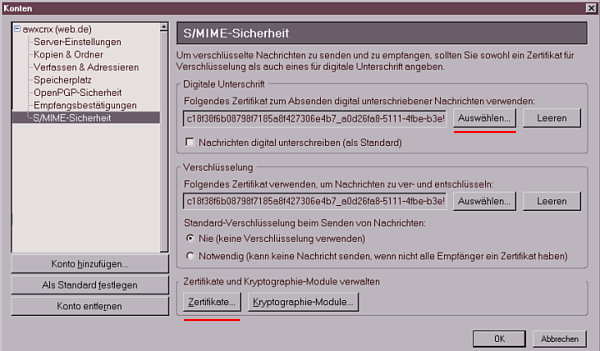
\includegraphics[scale=0.55]{../screenshots/thunderbird_smime_konto.png}
\caption{Kontoeinstellungen zur S/MIME-Sicherheit}
\label{abb:thunder_smime_konto}
\end{center}
\end{figure}

Zuerst ist das pers�nliche Zertifikat zu importieren. Ein Klick auf den Button \textit{Zertifikate} �ffnet den Manager f�r eigene Zertifikate (Bild \ref{abb:thunder_smime_zert}). Hier ist der Button \textit{Importieren} zu w�hlen und das gespeicherte pers�nliche Zertifikat mit �ffentlichem und geheimem Schl�ssel zu importieren.\\

\begin{figure}[htb]
\begin{center}
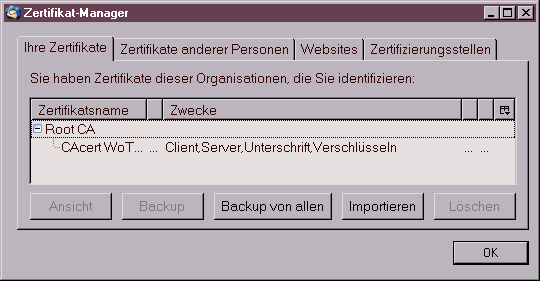
\includegraphics[scale=0.5]{../screenshots/thunderbird_einst_zert_3.png}
\caption{Zertifikatsmanager f�r eigene Zertifikate}
\label{abb:thunder_smime_zert}
\end{center}
\end{figure}

Es folgt eine Abfrage des Passwortes, mit dem der Zugriff auf den geheimen Schl�ssel gesch�tzt werden soll und evtl. die Frage nach dem Passwort, mit welchem die Datei verschl�sselt wurde. Der Zertifikatsmanager ist im Anschluss mit einem Klick auf den Button \textit{Ok} zu schlie�en und in den Konto-Einstellungen das frisch importierte Zertifikat f�r das Signieren und Entschl�sseln auszuw�hlen.\\

Sollen alle ausgehenden Nachrichten standardm��ig signiert werden, kann die entsprechende Option aktiviert werden.\\

Thunderbird bietet die M�glichkeit, das Online Certifate Status Protocol (OCSP) f�r die Validierung von Zertifikaten zu nutzen. Standardm��ig ist die Nutzung dieser Funktion sinnvoll deaktiviert. Da nur validierte Zertifikate f�r die Verschl�sselung und Signaturpr�fung genutzt werden k�nnen, muss man das Root Zertifikat der ausstellenden CA von der Website herunterladen und importieren. Dies kann vereinfacht werden, wenn man im Dialog \textit{Einstellungen} in der Sektion \textit{Datenschutz} auf dem Reiter \textit{Sicherheit} den Button \textit{OCSP...} w�hlt und die Option \textit{OCSP verwenden} aktiviert. Damit hat man jedoch keine M�glichkeit zu entscheiden, ob man der CA wirklich vertraut.

\subsection{Zertifikate der Partner und der CA importieren}
Im Gegensatz zu OpenPGP, das im Internet eine ausgereifte Infrastruktur zur Verteilung �ffentlicher Schl�ssel bereitstellt, muss der Inhaber eines S/MIME-Zertifikates selbst die Verteilung �bernehmen. Am einfachsten ist es, dem Partner eine signierte E-Mail zu senden. Alle E-Mail Clients mit S/MIME Support k�nnen aus der Signatur das Zertifikat importieren und tun dies in der Regel ohne Nachfrage.\\

Bevor der Empf�nger einer signierten E-Mail die Signatur pr�fen und verschl�sselt antworten kann, muss er das Zertifikat verifizieren. Viele Root-Zertifikate sind bereits in g�ngigen E-Mail Clients enthalten. Einige muss der Nutzer jedoch erst selbst importieren. Diese Root-Zertifikate stehen auf den Websites der Ausstellers zum Download bereit. Wurde die G�ltigkeit verifiziert, kann der Empf�nger im Anschlu� verschl�sselt antworten.\\

Es ist auch m�glich, eine Datei nur mit dem �ffentlichen Schl�ssel des Zertifikates auf den Rechner des Partners zu transferieren. Dort ist die Datei in Thunderbird zu importieren.\\

F�r den Import eines Zertifikates in Thunderbird ist der Dialog \textit{Einstellungen} zu �ffnen. In der Sektion \textit{Datenschutz} auf dem Reiter \textit{Sicherheit} ist der Button \textit{Zertifikate} zu w�hlen (Bild \ref{abb:thunder_smime_zert2}), um die Verwaltung zu �ffnen.\\

\begin{figure}[htb]
\begin{center}
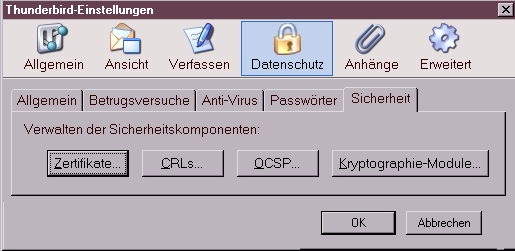
\includegraphics[scale=0.5]{../screenshots/thunderbird_einst_zert.png}
\caption{Dialog Sicherheits-Einstellungen}
\label{abb:thunder_smime_zert2}
\end{center}
\end{figure}

Im Zertifikatsmanager ist auf dem Reiter \textit{Zertifikate anderer Personen} der Button \textit{Importieren} zu finden, welcher eine Dateiauswahl �ffnet, um das erhaltene Zertifikat aus einer lokal gespeicherten Datei zu importieren.\\

Die Root-Zertifikate weiterer Certification Authorities (CAs) k�nnen auf dem Reiter \textit{Zertifizierungsstellen} importiert werden.

\subsection{Nachrichten verschl�sseln und signieren}
Wenn das pers�nliche Zertifikat bestehend aus �ffentlichem und geheimem Schl�ssel importiert wurde, ist es m�glich, signierte E-Mails zu versenden. Wurden Zertifikate mit den �ffentlichen Schl�sseln der Kommunikationspartner importiert, kann die Nachricht auch verschl�sselt werden.\\

\begin{figure}[htb]
\begin{center}
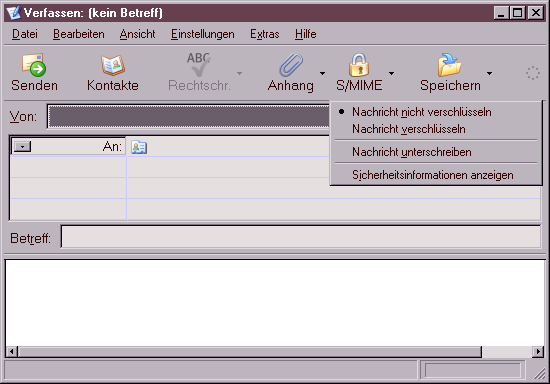
\includegraphics[scale=0.5]{../screenshots/thunderbird_smime_email.png}
\caption{Verschl�sseln oder Signieren einer E-Mail}
\label{abb:thunder_smime}
\end{center}
\end{figure}

F�r die Wahl der Optionen steht im Editor einer neuen Nachricht der Button S/MIME zur Verf�gung. Klickt man auf den kleinen schwarzen Pfeil unmittelbar neben dem Button S/MIME, �ffnet sich das im Bild \ref{abb:thunder_smime} dargestellte Men� zum Festlegen der Kryptographie-Optionen f�r die aktuelle Nachricht.\\

Eine M�glichkeit, f�r bestimmte Empf�nger die Einstellungen f�r Verschl�sselung dauerhaft festzulegen, bietet Thunderbird in der Standard-Konfiguration nicht. Man mu� bei jeder neu verfassten E-Mail daran denken, sie wenn m�glich zu verschl�sseln! Das ist sehr fehleranf�llig.\\

Eine L�sung bietet das Plug-In \textbf{Virtual Identity}. Es kann bei jeder versendeten E-Mail die gew�hlten Einstellungen f�r die Verschl�sselung speichern. Damit lernt Thunderbird, welche Verschl�sselungseinstellungen f�r welche Empf�nger gelten. Die Einstellungen werden bei jeder neuen E-Mail an den Empf�nger als Default aktiviert.\\

Nach der Installation des Plug-Ins muss man unter dem Men�punkt \textit{``Extras - Virtual Identity - Einstellungen''} die Speicherung der Einstellungen f�r die Verschl�sselung aktivieren. (Bild \ref{abb:vertual_id1})\\

\begin{figure}[htb]
\begin{center}
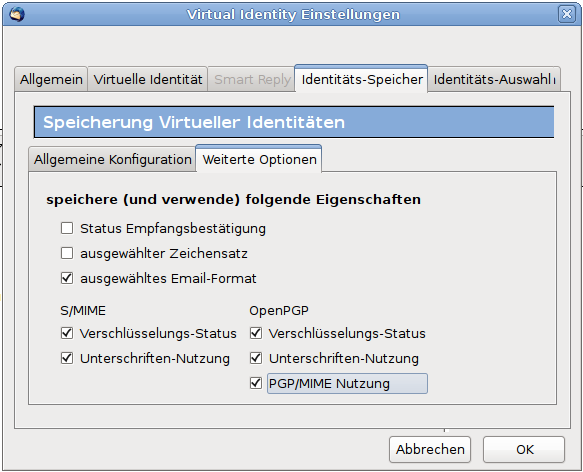
\includegraphics[scale=0.5]{../screenshots/virtual-id1.png}
\caption{Einstellungen des Plug-In Virtual Identity}
\label{abb:vertual_id1}
\end{center}
\end{figure}

Unter dem Men�punkt \textit{``Extras - Virtual Identity - Datenspeicher''} findet man die gesammelten Daten und kann sie auch editieren.
\section{Root-Zertifikate importieren}
Das Importieren der Zertifikate in Web-Browser und E-Mail-Client erspart l�stige Nachfragen, ob man einem mit diesem Root-Zertifikat signierten Zertifikat vertrauen m�chte.
\subsection{Webbrowser Firefox}
Nutzer des Browsers Firefox klicken auf auf das \textit{Root Certificate} und aktivieren in dem sich �ffnenden Dialog (Bild \ref{abb:firefox_ca_neu}) mindestens den ersten und zweiten Punkt.\\

\begin{figure}[htb]
 \begin{center}
  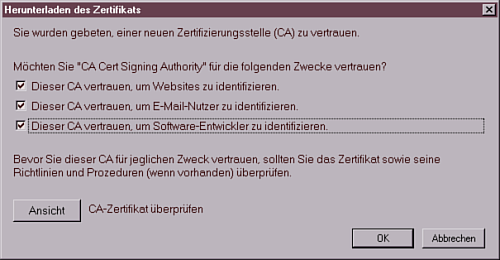
\includegraphics[scale=0.55]{../screenshots/cacert_certifikat.png}
  \caption{Herunterladen eines Zertifikates}
\label{abb:firefox_ca_neu}
 \end{center}
\end{figure}

\subsection{E-Mail-Client Thunderbird}
F�r den Import der Root-Zertifikate in den E-Mail-Client sind diese lokal zu speichern. In der Regel ben�tigt man neben dem \textit{Class 1 Root Certificate} auch das \textit{Class 3 Root Certificate}, da mit diesem Unterzertifikat die E-Mail-Zertifikate der Nutzer signiert werden. Nutzer des Browsers Firefox klicken mit der rechten Maustaste auf den Link und w�hlen aus dem Kontextmen� den Punkt \textit{Ziel speichern unter ...}\\

\begin{figure}[htb]
 \begin{center}
  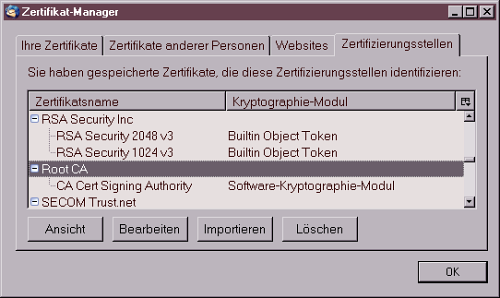
\includegraphics[scale=0.55]{../screenshots/thunderbird_zerti_manager.png}
  \caption{Zertifikats-Manager von Thunderbird}
\label{abb:thunder_ca_neu}
 \end{center}
\end{figure}

Anschlie�end ist Thunderbird zu starten und der Dialog \textit{Einstellungen} zu �ffnen. In der Sektion \textit{Datenschutz} / \textit{Sicherheit} ist der Button \textit{Zertifikate} zu w�hlen, um den in Bild \ref{abb:thunder_ca_neu} dargestellten Manager f�r Zertifikate zu �ffnen.\\

In diesem Dialog ist auf dem Reiter \textit{Zertifizierungsstellen} der Button \textit{Importieren} zu w�hlen und das zuvor gespeicherte Zertifikat zu importieren. Im Anschluss sind im folgenden Dialog mindestens die ersten beiden Optionen zu aktivieren (siehe Firefox).\\

\section{Eine eigene Certification Authority}
Wer eine eigene Certification Authority (CA) betreiben m�chte, ben�tigt etwas Erfahrung, einige kleine Tools und ein paar Byte Webspace, um das eigene Root-Zertifikate, die Revocation List und die Policy der CA dort zum Download bereitzustellen.\\

Die OpenSSL-Bibliothek enth�lt alle n�tigen Funktionen, um eine eigene CA zu verwalten. Die Hardcore Version auf der Kommandozeile hat M. Heimpold im Mini-Howto zur Zertifikatserstellung beschrieben.\\ \href{http://www.heimpold.de/mhei/mini-howto-zertifikaterstellung.htm}{http://www.heimpold.de/mhei/mini-howto-zertifikaterstellung.htm}.\\

Komfortabler geht es mit dem GUI TinyCA (\href{http://tinyca.sm-zone.net}{http://tinyca.sm-zone.net}). Die Website bietet eine Live-CD zum Download an, so dass ich mir weitere Ausf�hrungen zur Installation sparen kann. Unter Debian GNU/Linux kann man das Tool mit Apt installieren:

\begin{verbatim}
   # apt-get install tinyca
\end{verbatim}

Nach dem Start mit dem Kommando \textit{tinyca2} werden in zwei Dialogen die Angaben zum Root-Zertifikat der CA abgefragt. Da TinyCA mehrere CAs verwaltet, kann man erst einmal mit einem Test beginnen.\\

\begin{figure}[htb]
 \begin{center}
  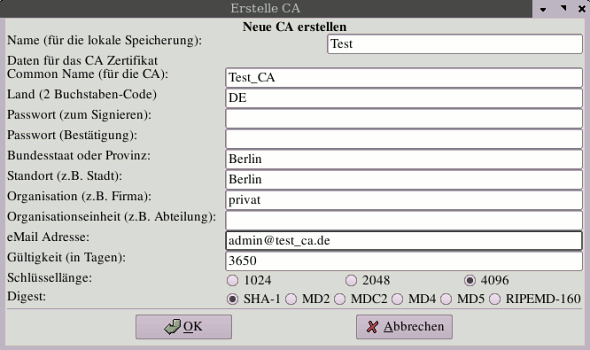
\includegraphics[scale=0.55]{../screenshots/tinyca1.png}
  \caption{Anlegen einer neuen CA}
\label{abb:tinyca1}
 \end{center}
\end{figure}

Der \textit{Common Name} der CA kann frei gew�hlt werden. Das Passwort sollte man sich gut �berlegen und keinesfalls vergessen. Mit einem Klick auf \textit{Ok} erscheint ein zweiter Dialog mit weiteren Angaben zur CA. Wichtig sind hier die URL der Revocation List f�r zur�ckgezogene Zertifikate und die URL der Policy der CA. Die Policy ist ein HTML-Dokument, welches beschreibt, wer ein Zertifikat von dieser CA erhalten kann, also z.B. etwas in der Art: \textit{Nur f�r pers�nlich Bekannte!}\\

Im Anschluss k�nnen die E-Mail Zertifikate der Nutzer erstellt werden. Die n�tigen Angaben sind selbsterkl�rend (Bild \ref{abb:tinyca3}. Mit einem Klick auf \textit{Ok} wird das S/MIME-Zertifikat erstellt und mit dem Root-Zertifikat der CA signiert. Dabei wird das Password f�r den geheimen Key der CA abgefragt.\\

\begin{figure}[htb]
 \begin{center}
  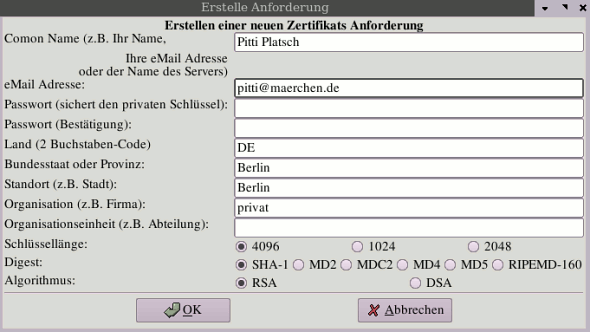
\includegraphics[scale=0.55]{../screenshots/tinyca3.png}
  \caption{Erstellen eines E-Mail Zertifikats}
\label{abb:tinyca3}
 \end{center}
\end{figure}

Um einem Nutzer sein Zertifikat zur Verf�gung zu stellen, ist es in eine Datei zu exportieren. Das PKCS\#12-Format (*.p12) enth�lt den geheimen und den �ffentlichen Schl�ssel, ist mit einem Passwort gesichert und kann von allen E-Mail Clients importiert werden.\\

\begin{figure}[htb]
 \begin{center}
  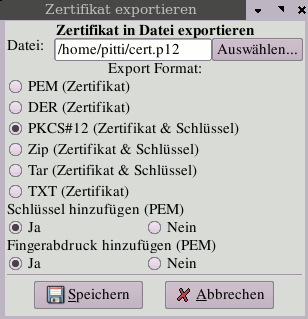
\includegraphics[scale=0.5]{../screenshots/tinyca5.png}
  \caption{Zertifikat exportieren}
\label{abb:tinyca5}
 \end{center}
\end{figure}

Das Root-Zertifikat der CA ist als DER- oder PEM-Format zu exportieren. Diese Datei enth�lt nur den �ffentlichen Schl�ssel des Zertifikates und kann zum Download bereitgestellt werden. Au�erdem ist regelm��ig eine Revocation List mit abgelaufenen oder zur�ckgezogenen Zertifikaten zu erstellen und ebenfalls zum Download unter der angegebenen URL bereitzustellen. Die Oberfl�che bietet f�r beide Aufgaben einen Button in der Toolbar.
\section{Ist S/MIME-Verschl�sselung unsicher?}
Nach unserer Einsch�tzung ist die S/MIME-Verschl�sselung wesentlich schw�cher, als OpenPGP. Die Ursachen liegen nicht in einer Schw�che der verwendeten Algorithmen, sondern in der Generierung und Speicherung der privaten Schl�ssel au�erhalb der Hoheit des Anwenders.\\

Die Sicherheit asymmetrischer Kryptografie h�ngt entscheidend von der Vertrauensw�rdikeit der privaten Schl�ssel ab. W�hrend der �ffentliche Schl�ssel m�glichst breit zu verteilen ist, muss die Verf�gungsgewalt f�r den privaten Schl�ssel ausschlie�lich und vollst�ndig(!) in der Hand des Anwenders liegen. Nur so kann gew�hrleistet werden, dass kein unbefugter Dritter die vertrauliche Kommunikation entschl�sseln kann.\\

Um die Nutzung der S/MIME-Verschl�sselung f�r unbedarfte Anwender zu erleichtern, wird die Erzeugung und Aufbewahrung der privaten Schl�ssel h�ufig durch organisatorische Schw�chen kompromittiert.

\subsubsection*{Erzeugen der privaten Keys}
Alle Anbieter von Zertifizierungen f�r X.509 Zertifikate bieten eine webbasiertes Interface f�r die Erzeugung und Signatur der Zertifikate. In der Regel werden nach erfolgricher �berpr�fung der Identit�t des Antragstellers zwei Varianten f�r die Generierung eines g�ltigen Zertifikates angeboten: 
\begin{enumerate}
 \item Man kann nach in einer selbst gew�hlten sicheren Umgebung den privaten Schl�ssel und ein Certification Request (CSR) erzeugen. Der CSR enth�lt nur den �ffentlich Schl�ssel. Dieser wird im Webinterface hochgeladen und man erh�lt via E-Mail oder Download Link das signierte Zertifikat.
 \item Man die komplette Generierung des privaten und �ffentlichen Schl�ssels der CA �berlassen und muss darauf vertrauen, dass dieser keine Kopie des privaten Schl�ssels speichert.
\end{enumerate}

Aus Bequemlichkeit nutzt die absolute Mehrheit der Anwender den 2. Weg und geht damit das Risiko ein, dass die Schl�ssel bereits vor der Verwendung kompromittiert werden k�nnte.\\ 

In einem Forschungspapier kommen die Sicherheitsforscher C. Soghoian und S. Stamm zu dem Schluss, das die US-Regierung von kooperierenden Certification Authorities die privaten Keys von X509-Zertifikaten erhalten k�nnte und die US-Beh�rden somit die Daten problemlos entschl�sseln k�nnen. Eine �hnliche Zusammenarbeit gibt es unserer Meinung nach auch zwischen Startcom-SSL und dem isrealischen Geheimdienst.

\subsubsection*{Der Deutsche Bundestag}
Der Deutsche Bundestag bietet allen Abgeordneten die M�glichkeit, S/MIME f�r die Verschl�sselung von E-Mails zu verwenden.\\

Die Abgeordneten sind scheinbar nicht �ber diese M�glichkeit informiert. Bei der technischen Umsetzung gilt das Prinzip \textit{Security by obscurity}, wie ein Testbericht zeigt (\href{http://www.heise.de//tp/r4/artikel/27/27182/1.html}{http://www.heise.de//tp/r4/artikel/27/27182/1.html}).\\

Um die Abgeordneten maximal von der ``komplizierten'' Technik des Entschl�sseln der E-Mail zu entlasten, erfolgt die Entschl�sselung auf einem zentralen Server des Bundestages. Auf diesem zentralen Server liegen auch die privaten Schl�ssel und die Zertifikate der Abgeordneten.\\

Damit ist gesichert, dass auch die Sekret�rinnen keine Probleme haben, wenn der Absender einer E-Mail diese verschl�sselt und damit sicherstellen wollte, dass nur der Abgordnete selbst sie lesen kann.\\

Hier wird eine Vertraulichkeit der Kommunikation vorgegaukelt. Gef�hrlich wird dieser Placebo, wenn ein B�rger auf die Sicherheit vertraut und sich gegen�ber seinem Abgeordneten freim�tiger �u�ert, als er es unverschl�sselt tun w�rde.

\subsubsection*{Web.de (Free-) Mail-Account}
Beim Anlegen eines Mail-Accounts bei Web.de wird automatisch ein S/MIME-Zertifikat f�r den Nutzer generiert. Der �ffentliche und der private Schl�ssel liegen auf dem Server des Anbieters. Der Schl�ssel ist nicht durch ein Passwort gesch�tzt.\\

Dieses Feature wird von Web.de wie folgt beworben:\\

\textit{``Versehen Sie Ihre E-Mail mit einer digitalen Unterschrift, kann diese auf dem Weg zum Empf�nger nicht ver�ndert werden. Die digitale Verschl�sselung sorgt daf�r, dass die E-Mail auf dem Weg zum Empf�nger nicht gelesen werden kann.''}\\

Au�erdem fordert die Website dazu auf, das Zertifikat im eigenen E-Mail Client zu importieren und f�r die Verschl�sselung zu nutzen.\\

Diese Variante von S/MIME ist ein Placebo, den man ignorieren sollte.\\

Die Werbebotschaft entspricht nicht der Wahrheit. Gem�� geltendem Recht ist die E-Mail beim Empf�nger angekommen, wenn der Empf�nger Gelegenheit hatte, sie zur Kenntnis zu nehmen. Vorher kann sie jedoch auf dem Server von Web.de entschl�sselt werden (auch von stattlichen Stellen).

\subsubsection*{Projekt De-Mail}
Auch das geplante Portale De-Mail f�r die rechtsverbindliche und sichere deutsche Alternative zur E-Mail soll X.509 Zertifikate f�r die Gew�hrleistung der vertraulichen Kommunikation nutzen. Die Anforderungen sehen eine Entschl�sselung der vertraulichen E-Mails durch Betreiber des Dienstes ausdr�cklich vor. Als Grund wird die Notwendigkeit des Virescans genannt.\\

Au�erdem wirbt das Projekt damit, den Nutzern einen ``Datentresor'' f�r vertrauliche digitale Dokumente zur Verf�gung zu stellen. Das Konzept kann jedoch nur als Placebo bezeichnet werden. Sowohl die verschl�sselten Dokumente als auch die Schl�ssel f�r den Zugriff auf die Dokumente sollen beim Anbieter des Dienstes liegen. Die Entschl�sselung der vertraulichen Daten durch Mitarbeiter ist ebenfalls ausdr�cklich vorgesehen.\\

Das Projekt De-Mail wird in Zusammenarbeit mit dem ePA einen Key-Escrow (Hinterlegung der Schl�ssel bei den Beh�rden) f�r unbedarfte Anwender vorrantreiben. Den Anwendern wird eine Sicherheit vorgegaukelt, die durch Beh�rden einfach kompromittiert werden kann.

\subsubsection*{Schlu�folgerung}
Im Gegensatz zu OpenPGP kann man bei S/MIME nicht sicher davon ausgehen, dass der Gegen�ber seinen privaten Schl�ssel selbst generiert hat und dass der Schl�ssel ausschlie�lich ihm zur Verf�gung steht.
Es besteht damit die Gefahr, dass die Vertraulichkeit der Kommunikation nicht umfassend gew�hrleistet ist.\\

In extremen F�llen ist die angebotene Verschl�sselung nur ein Placebo.\\

Staatliche Projekte wie der ePA zusammen mit dem Projekt De-Mail weichen die Sicherheit der S/MIME Verschl�sselung weiter auf.
\section{Eine Bemerkung zum Abschlu�}
\textit{``Mache ich mich verd�chtig, wenn ich meine E-Mails verschl�ssel?''}\\

Eine Frage, die h�ufig gestellt wird, wenn es um verschl�sselte E-Mails geht. Bisher gab es darauf folgende Antwort:\\

\textit{``Man sieht es einer E-Mail nicht an, ob sie verschl�sselt ist oder nicht. Wer bef�rchtet, dass jemand die Mail beschn�ffelt und feststellen k�nnte, dass sie verschl�sselt ist, hat einen Grund mehr, kryptografische Verfahren zu nutzen!''}\\

Aktuelle Ereignisse zeigen, dass diese Frage nicht mehr so einfach beantwortet werden kann. Dem promovierten Soziologen Andrej H. wurde vorgeworfen, Mitglied einer terroristischen Vereinigung nach �129a StGB zu sein. Der Haftbefehl gegen ihn wurde unter anderem mit \textbf{konspirativem Verhalten} begr�ndet, da er seine E-Mails verschl�sselte.\\

Am 21.Mai 2008 wurden in �stereich die Wohnungen von Aktivisten der Tierrechtsszene durchsucht und 10 Personen festgenommen. Der Haftbefehl wurde mit Verdunklungsgefahr begr�ndet, da die Betroffenen z.B. �ber verschl�sselte E-Mails kommunizierten.\\

Am 18.10.07 hat der Bundesgerichtshof (BGH) in seinem Urteil \href{http://juris.bundesgerichtshof.de/cgi-bin/rechtsprechung/document.py?Gericht=bgh&Art=pm&Datum=2007&Sort=3&anz=154&pos=0&nr=41487&linked=bes&Blank=1&file=dokument.pdf}{Az.: StB 34/07} den Haftbefehl gegen Andrej H. aufgehoben und eindeutig festgestellt, dass die Verschl�sselung von E-Mails als Tatverdacht NICHT ausreichend ist, entscheidend sei der Inhalt: \\

\textit{``Ohne eine Entschl�sselung der in den Nachrichten verwendeten Tarnbegriffe und ohne Kenntnis dessen, was bei den - teilweise observierten und auch abgeh�rten - Treffen zwischen dem Beschuldigten und L. besprochen wurde, wird hierdurch eine mitgliedschaftliche Einbindung des Beschuldigten in die 'militante gruppe' jedoch nicht hinreichend belegt.''}\\

Au�erdem geben die Richter des 3. Strafsenat des BGH zu bedenken, dass Andrej H. \textit{``ersichtlich um seine �berwachung durch die Ermittlungsbeh�rden wusste''}. Schon allein deshalb konnte er \textit{``ganz allgemein Anlass sehen''}, seine Aktivit�ten zu verheimlichen. Woher Andrej H. von der �berwachung wusste, steht bei \href{http://annalist.noblogs.org/}{http://annalist.noblogs.org}.\\

Trotz dieses Urteils des BGH bleibt f�r uns ein bitterer Nachgeschmack �ber die Arbeit unser Ermittler und einiger Richter. Zumindest die Ermittlungsrichter sind der Argumentation der Staatsanwaltschaft gefolgt und haben dem Haftbefehl erst einmal zugestimmt.

\end{document}